\documentclass[tikz,border=6pt]{standalone}
\usepackage{times}
\usepackage{pgfplots}
\pgfplotsset{compat=1.18}
\begin{document}
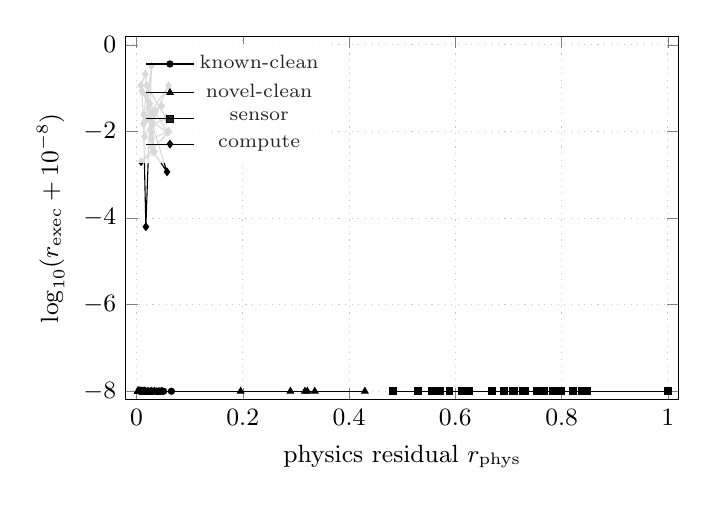
\begin{tikzpicture}
\begin{axis}[
  width=8.6cm, height=6.2cm,
  xlabel={physics residual $r_{\mathrm{phys}}$},
  ylabel={$\log_{10}(r_{\mathrm{exec}}+10^{-8})$},
  xmin=-0.02, xmax=1.02,
  ymin=-8.2, ymax=0.2,
  legend style={at={(0.02,0.98)}, anchor=north west, font=\scriptsize, draw=none, fill=white, fill opacity=0.85},
  grid=major, major grid style={dotted, gray!45},
  tick label style={font=\small}, label style={font=\small},
]
\addplot[mark=*, mark size=1.1pt] coordinates { (0.0199,-8.0000) (0.0122,-8.0000) (0.0402,-8.0000) (0.0475,-8.0000) (0.0279,-8.0000) (0.0256,-8.0000) (0.0417,-8.0000) (0.0181,-8.0000) (0.0128,-8.0000) (0.0129,-8.0000) (0.0430,-8.0000) (0.0062,-8.0000) (0.0225,-8.0000) (0.0482,-8.0000) (0.0083,-8.0000) (0.0318,-8.0000) (0.0145,-8.0000) (0.0442,-8.0000) (0.0119,-8.0000) (0.0656,-8.0000) (0.0510,-8.0000) (0.0442,-8.0000) (0.0270,-8.0000) (0.0384,-8.0000) (0.0365,-8.0000) (0.0141,-8.0000) (0.0170,-8.0000) (0.0305,-8.0000) };\addlegendentry{known-clean}
\addplot[mark=triangle*, mark size=1.3pt] coordinates { (0.0159,-8.0000) (0.0044,-8.0000) (0.0142,-8.0000) (0.0058,-8.0000) (0.0333,-8.0000) (0.0274,-8.0000) (0.0215,-8.0000) (0.0152,-8.0000) (0.0023,-8.0000) (0.0031,-8.0000) (0.0477,-8.0000) (0.0064,-8.0000) (0.4297,-8.0000) (0.0076,-8.0000) (0.0031,-8.0000) (0.0036,-8.0000) (0.0034,-8.0000) (0.2896,-8.0000) (0.0060,-8.0000) (0.3215,-8.0000) (0.0042,-8.0000) (0.3169,-8.0000) (0.3355,-8.0000) (0.1960,-8.0000) (0.0096,-8.0000) (0.0049,-8.0000) (0.0121,-8.0000) (0.0094,-8.0000) };\addlegendentry{novel-clean}
\addplot[mark=square*, mark size=1.2pt] coordinates { (0.8214,-8.0000) (0.6128,-8.0000) (1.0000,-8.0000) (0.7831,-8.0000) (0.7602,-8.0000) (0.6693,-8.0000) (1.0000,-8.0000) (0.6910,-8.0000) (0.6253,-8.0000) (0.5708,-8.0000) (0.5303,-8.0000) (0.7853,-8.0000) (0.5890,-8.0000) (0.4820,-8.0000) (0.7663,-8.0000) (1.0000,-8.0000) (0.7543,-8.0000) (0.7103,-8.0000) (0.7312,-8.0000) (0.7080,-8.0000) (0.8389,-8.0000) (0.8475,-8.0000) (0.8474,-8.0000) (0.7985,-8.0000) (0.5554,-8.0000) (0.7270,-8.0000) (1.0000,-8.0000) (0.6148,-8.0000) };\addlegendentry{sensor}
\addplot[mark=diamond*, mark size=1.3pt] coordinates { (0.0472,-1.4107) (0.0132,-1.8233) (0.0176,-4.2008) (0.0282,-0.4856) (0.0165,-1.7445) (0.0606,-0.9402) (0.0151,-2.1179) (0.0100,-1.0688) (0.0310,-1.5748) (0.0202,-1.6975) (0.0585,-2.0215) (0.0254,-1.3530) (0.0086,-0.9371) (0.0166,-0.6746) (0.0338,-2.4683) (0.0087,-2.6969) (0.0608,-1.9999) (0.0278,-2.1704) (0.0280,-1.7782) (0.0573,-2.9313) (0.0322,-2.4760) (0.0191,-0.9359) (0.0557,-1.6937) (0.0292,-1.8442) (0.0136,-1.6072) (0.0185,-1.1589) (0.0286,-2.3563) (0.0361,-1.5303) };\addlegendentry{compute}
\end{axis}
\end{tikzpicture}
\end{document}
